%%%%%%%%%%%%%%%%%%%%%%%%%%%%%%%%%%%%%%%%%%%%%%%%%%%%%%%%%%%%%%%%%%%%%%
% CS638: Applied Machine Learning
% Copyright 2016 Pejman Ghorbanzade <pejman@ghorbanzade.com>
% Creative Commons Attribution-ShareAlike 4.0 International License
% More info: https://github.com/ghorbanzade/beacon
%%%%%%%%%%%%%%%%%%%%%%%%%%%%%%%%%%%%%%%%%%%%%%%%%%%%%%%%%%%%%%%%%%%%%%

\def \topDirectory {.}
\def \srcDirectory {\topDirectory/src}
\def \texDirectory {\srcDirectory/tex}
\def \imgDirectory {\topDirectory/../build/umb-cs638-2016s/img}

\documentclass[compress]{beamer}
\mode<presentation>
\usetheme{default}

\usepackage{enumitem}
\usepackage[font=scriptsize]{caption}

\date{\today}
\title{Real-Time Human Physical Activity Recognition}
\subtitle{Project Proposal for CS638 Applied Machine Learning}
\author[pejman]{Pejman Ghorbanzade\\ \texttt{pejman@cs.umb.edu}}
\institute[UMass]{Department of Computer Science\\ University of Massachusetts Boston}

\setbeamertemplate{navigation symbols}{}

\setbeamertemplate{footline}[text line]{
	\parbox{\linewidth}{\vspace*{-10pt}\hfill Pejman Ghorbanzade}
}

\begin{document}

\begin{frame}
	\frametitle{\inserttitle}
	\framesubtitle{\insertsubtitle}

	\emph{Objective} Identify human physical activities of daily living using a network of wearable motion sensors.

	\begin{columns}
	\column{0.6\textwidth}

	\begin{figure}
	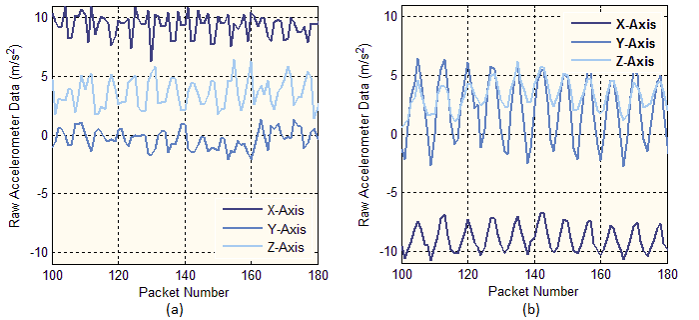
\includegraphics[width=\textwidth]{\texDirectory/hw01-plot.png}
	\caption{Acceleration data of a single node during (a) walking and (b) waving}
	\end{figure}

	\column{0.4\textwidth}

	\footnotesize

	\emph{Dataset Characteristics}
	\begin{itemize}[leftmargin=10pt]
	\item[] 8 motion sensors
	\item[] 10 subjects
	\item[] 30 activities
	\end{itemize}

	\emph{Proposed Algorithms}
	\begin{itemize}[leftmargin=10pt]
	\item[] Support Vector Machine
	\item[] Hidden Markov Model
	\end{itemize}

	\end{columns}

\end{frame}

\end{document}
